\documentclass{article}

\usepackage[latin1]{inputenc}
\usepackage{tikz}
\usepackage[papersize={15cm,9cm},left=-.15cm,right=.5cm,bottom=.1cm,top=.1cm]{geometry}
\usetikzlibrary{shapes,arrows}
\begin{document}
\pagestyle{empty}

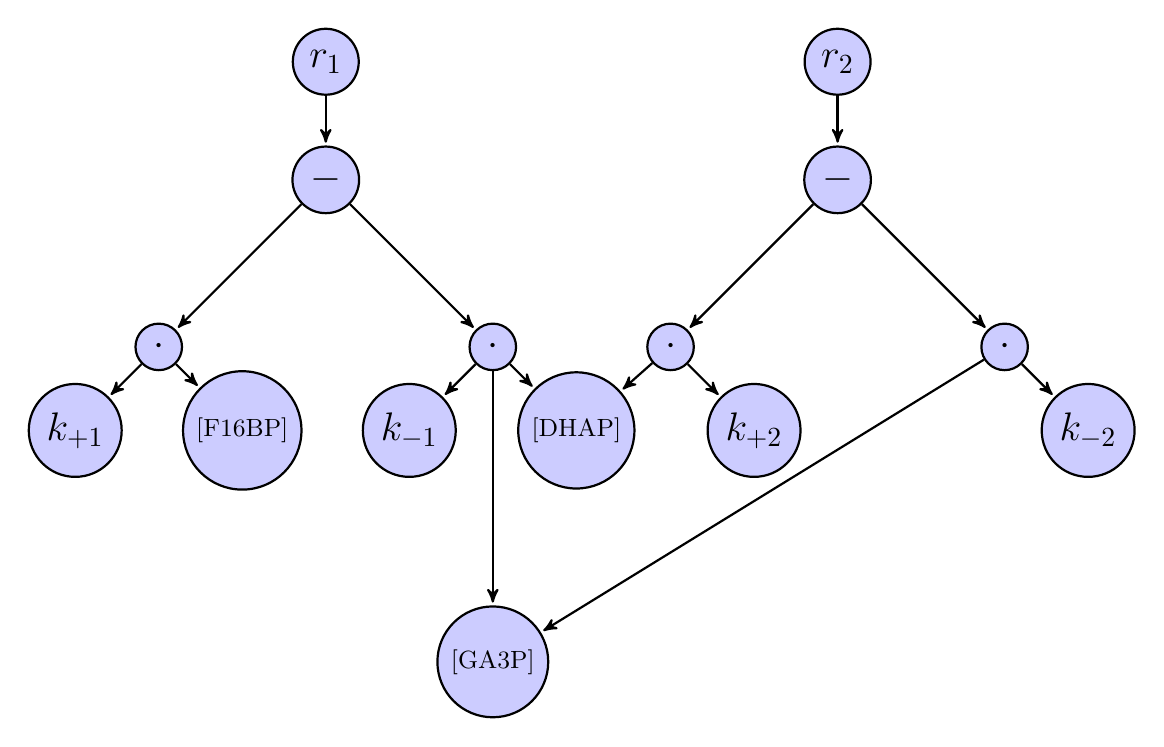
\begin{tikzpicture}[->,>=stealth',shorten >=1pt,auto,node distance=1.5cm,
  thick,main node/.style={circle,fill=blue!20,draw,font=\sffamily\Large\bfseries}]

  \node[main node] (r1) {$r_{1}$};
  \node[main node] (r2) [right of=r1, node distance = 6.5cm] {$r_{2}$};
  
  \node[main node] (minus1) [below of=r1] {$-$};
  \node[main node] (times1) [node distance = 3cm] [below left of=minus1] {$\cdot$};
  \node[main node] (kass1) [below left of=times1] {$k_{+1}$};
\node[main node]  [font=\small] (F16BP) [below right of=times1] {[F16BP]};

\node[main node] (times2)  [node distance = 3cm] [below right of=minus1] {$\cdot$};
\node[main node] (kdiss1) [below left of=times2] {$k_{-1}$};
\node[main node]  [font=\small] [node distance = 4cm] (GA3P) [below of=times2] {[GA3P]};
\node[main node]  [font=\small] (DHAP) [below right of=times2] {[DHAP]};

  \node[main node] (minus2) [below of=r2] {$-$};
\node[main node] (times3) [node distance = 3cm] [below left of=minus2] {$\cdot$};
  \node[main node] (kass2) [below right of=times3] {$k_{+2}$};

\node[main node] (times4)[node distance = 3cm] [below right of=minus2] {$\cdot$};
\node[main node] (kdiss2) [below right of=times4] {$k_{-2}$};
 \path[every node/.style={font=\sffamily\small}]
    (r1) edge (minus1)
    (minus1) edge (times1)
    (minus1) edge (times2)
    (times1) edge (kass1)
   (times1) edge (F16BP)
(times2) edge (kdiss1)
   (times2) edge (GA3P)
  (times2) edge (DHAP)
  (r2) edge (minus2)
    (minus2) edge (times3)
    (minus2) edge (times4)
 (times3) edge (kass2)
   (times3) edge (DHAP)
 (times4) edge (kdiss2)
   (times4) edge (GA3P);
       \end{tikzpicture}
\end{document}